% Diagrama de arquitectura — Rendir.ai (TikZ standalone)
% Compilar: pdflatex arquitectura.tex  ->  arquitectura.pdf  ->  PNG (PyMuPDF)
\documentclass[border=16pt]{standalone}
\usepackage[T1]{fontenc}
\usepackage[utf8]{inputenc}
\usepackage[sfdefault]{FiraSans}
\usepackage{tikz}
\usetikzlibrary{positioning,arrows.meta}

\definecolor{amber}{HTML}{F08C00}
\definecolor{amberdeep}{HTML}{C2410C}
\definecolor{ink}{HTML}{2B2118}
\definecolor{panel}{HTML}{FBEEDD}
\definecolor{cream}{HTML}{FFFCF7}

\begin{document}
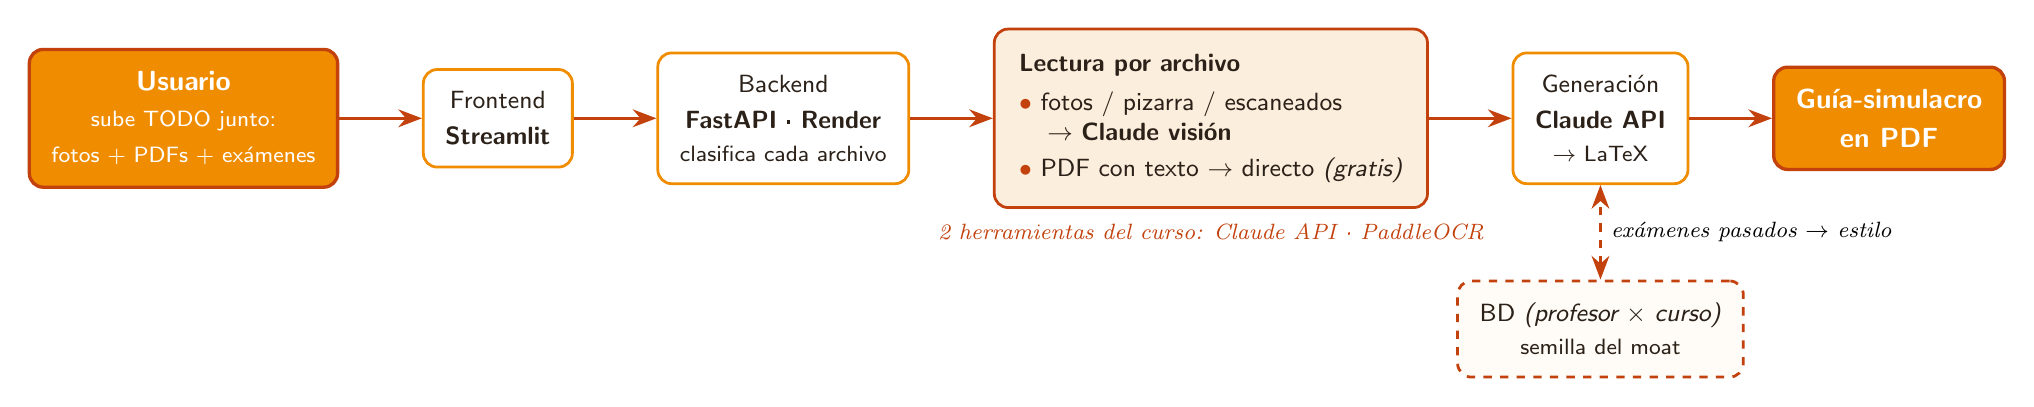
\begin{tikzpicture}[
  font=\sffamily\small,
  >={Stealth[length=3mm]},
  node distance=1.05cm,
  box/.style ={rounded corners=5pt, draw=amber, line width=1pt, fill=white,
               text=ink, align=center, inner sep=8pt, minimum height=1.2cm},
  hd/.style  ={rounded corners=5pt, draw=amberdeep, line width=1.2pt, fill=amber,
               text=white, align=center, inner sep=8pt, minimum height=1.2cm,
               font=\sffamily\bfseries},
  read/.style={rounded corners=5pt, draw=amberdeep, line width=1pt, fill=panel,
               text=ink, align=left, inner sep=9pt, minimum height=1.2cm},
  store/.style={rounded corners=5pt, draw=amberdeep, line width=1pt, dashed,
               fill=cream, text=ink, align=center, inner sep=8pt},
  flow/.style ={->, draw=amberdeep, line width=1.1pt},
  dashflow/.style ={<->, draw=amberdeep, line width=1pt, dashed},
]
  % --- fila principal (pipeline) ---
  \node[hd]   (user)  {Usuario\\[1pt]{\footnotesize\mdseries sube TODO junto:}\\[1pt]{\footnotesize\mdseries fotos + PDFs + exámenes}};
  \node[box, right=of user]  (front) {Frontend\\[2pt]\textbf{Streamlit}};
  \node[box, right=of front] (back)  {Backend\\[2pt]\textbf{FastAPI · Render}\\[1pt]{\footnotesize clasifica cada archivo}};
  \node[read, right=of back] (lect)  {\textbf{Lectura por archivo}\\[3pt]
        \textcolor{amberdeep}{$\bullet$} fotos / pizarra / escaneados\\ \hspace{1.1em}$\to$ \textbf{Claude visión}\\[2pt]
        \textcolor{amberdeep}{$\bullet$} PDF con texto $\to$ directo \emph{(gratis)}};
  \node[box, right=of lect]  (gen)   {Generación\\[2pt]\textbf{Claude API}\\[1pt]{\footnotesize $\to$ LaTeX}};
  \node[hd,  right=of gen]   (pdf)   {Guía-simulacro\\[2pt]\textbf{en PDF}};

  % --- moat (dataset) ---
  \node[store, below=1.2cm of gen] (moat) {BD \textit{(profesor $\times$ curso)}\\[1pt]{\footnotesize semilla del moat}};

  % --- flechas ---
  \draw[flow] (user)  -- (front);
  \draw[flow] (front) -- (back);
  \draw[flow] (back)  -- (lect);
  \draw[flow] (lect)  -- (gen);
  \draw[flow] (gen)   -- (pdf);
  \draw[dashflow] (moat)  -- (gen) node[midway, right, font=\footnotesize\itshape] {exámenes pasados $\to$ estilo};

  % --- herramientas del curso (etiquetas) ---
  \node[font=\footnotesize\itshape\color{amberdeep}, below=2pt of lect.south] {2 herramientas del curso: Claude API · PaddleOCR};
\end{tikzpicture}
\end{document}
